\documentclass[11pt]{article}
\usepackage[margin=1in]{geometry}
\usepackage{amsmath,amssymb}
\usepackage{booktabs}
\usepackage{enumitem}
\usepackage{graphicx}
\usepackage{xcolor}
\usepackage{float}

% \ans{...}: wrap each final answer so it stands out for the grader.
\newcommand{\ans}[1]{$\boxed{#1}$}
% \todo{...}: placeholder text, shown in grey. Delete each one as you fill it in.
\newcommand{\todo}[1]{\textcolor{gray}{[#1]}}

\setlength{\parindent}{0pt}
\setlength{\parskip}{6pt}

\title{Economics 2200 --- Homework 1}
\author{Ian Lent}
\date{October 6, 2026}

\begin{document}
\maketitle

%==================================================================
\section{GDP Per Capita in the United Kingdom}
%==================================================================

\begin{enumerate}[label=\textbf{\arabic*.}, leftmargin=*]

\item \textbf{Annual growth rates, 2006--2009 and 2019--2022.}
Growth rate $=y_{t+1}/y_t-1$.

\begin{table}[H]\centering
\begin{tabular}{lc}
\toprule
Period & Growth rate of GDP pc \\
\midrule
2006--2007 & \ans{+1.67\%} \\
2007--2008 & \ans{-1.50\%} \\
2008--2009 & \ans{-5.14\%} \\
2019--2020 & \ans{-11.41\%} \\
2020--2021 & \ans{+7.17\%} \\
2021--2022 & \ans{+3.43\%} \\
\bottomrule
\end{tabular}
\end{table}

\emph{2006--2009:} Growth was positive in 2007 but turned negative in 2008 and sharply so in 2009, which is the Global Financial Crisis (banking crisis, credit crunch and the ensuing Great Recession). UK GDP pc fell by roughly 5\% in 2009, reflecting collapsing financial-sector activity, investment and trade.

\emph{2019--2022:} The 11\% fall in 2020 reflects the COVID-19 pandemic and the lockdowns that shut down large parts of the economy. The rebound in 2021 (+7.2\%) and 2022 (+3.4\%) reflects reopening and vaccination plus fiscal and monetary support, though by 2022 GDP pc was still just below its 2019 level.

\item \textbf{Constant growth rate, 1000--1500.}
\[
  y_{1500} = (1+g)^{500}\, y_{1000}
  \quad\Longrightarrow\quad
  g = \left(\frac{y_{1500}}{y_{1000}}\right)^{1/500} - 1
    = \left(\frac{1697}{1151}\right)^{1/500} - 1 = 0.000777
\]
\ans{g \approx 0.078\%\ \text{per year}}

\item \textbf{Constant growth rate, 1500--1820.}
\[
  g = \left(\frac{3306}{1697}\right)^{1/320} - 1 = (1.9481)^{1/320}-1 = 0.002086
\]
\ans{g \approx 0.21\%\ \text{per year}}

\item \textbf{Constant growth rate, 1820--1950.}
\[
  g = \left(\frac{11061}{3306}\right)^{1/130} - 1 = (3.3457)^{1/130}-1 = 0.009333
\]
\ans{g \approx 0.93\%\ \text{per year}}

\item \textbf{Constant growth rate, 1950--2019.}
\[
  g = \left(\frac{39113}{11061}\right)^{1/69} - 1 = (3.5361)^{1/69}-1 = 0.018473
\]
\ans{g \approx 1.85\%\ \text{per year}}

\item \textbf{Dating the start of sustained growth.}
Growth was essentially zero (0.08\% per year) from 1000 to 1500, rose slightly to 0.21\% over 1500--1820, then jumped to 0.93\% over 1820--1950 (more than four times the earlier rate) and 1.85\% after 1950. Growth rates this high, sustained, are only seen from around 1820 onward, so I would date the start of sustained growth (the Industrial Revolution) at roughly \ans{\text{around 1800--1820}}. The 1500--1820 rate is already a bit higher than before, suggesting the acceleration began in the late 18th century.

\item \textbf{Counterfactual GDP pc in 2022 at the 1000--1500 rate.}
From 1820 to 2022 is 202 years:
\[
  y_{2022}^{cf} = 3306\,(1.000777)^{202} = 3306 \times 1.170 \approx 3{,}867
\]
\ans{y_{2022} \approx \$3{,}867}
This is about one tenth of the actual 2022 value of \$38,407.

\item \textbf{Implied GDP pc in 1000 at the 1950--2019 rate.}
From 1000 to 2022 is 1022 years, so
\[
  y_{1000} = \frac{y_{2022}}{(1.018473)^{1022}} = \frac{38407}{(1.018473)^{1022}} \approx 0.00029
\]
\ans{y_{1000} \approx \$0.0003 \ (\text{less than a thousandth of a dollar})}

Conclusion: An income of a fraction of a cent per year is impossible (people could not survive), whereas actual income in 1000 was \$1,151. Hence growth at today's rate cannot have prevailed throughout history: growth of 1--2\% per year is a very recent phenomenon, and for most of history growth was close to zero.

\item \textbf{Year in which UK GDP pc triples its 2022 value.}
Need $(1.018473)^t = 3$, so
\[
  t = \frac{\ln 3}{\ln 1.018473} = \frac{1.0986}{0.018304} \approx 60.0 \text{ years}
\]
\ans{\text{Year} \approx 2082}

\item \textbf{First year India's GDP pc exceeds the UK's.}
Need $7766\,(1.05)^t > 38407\,(1.018473)^t$:
\[
  t > \frac{\ln(38407/7766)}{\ln 1.05 - \ln 1.018473}
    = \frac{1.5985}{0.04879 - 0.01830} \approx 52.4 \text{ years}
\]
So the first full year is $t=53$.
\ans{\text{Year} \approx 2075}

\item \textbf{UK inflation, 2021--2022.}
Real GDP pc grew by $g_{y} = 38407/37134 - 1 = 3.43\%$. Real GDP growth is (approximately) pc growth plus population growth: $(1.0343)(1.01) = 1.0446$, i.e.\ about 4.46\%. Nominal GDP growth equals real growth times the price level growth: $1.06 = (1.0446)(1+\pi)$, so
\[
  1+\pi = \frac{1.06}{(1.0343)(1.01)} = 1.0147
\]
Exact calculation, no approximation needed. (Approximation: $\pi \approx 6\% - 1\% - 3.43\% = 1.57\%$, using $\ln(1+x)\approx x$.)

\ans{\pi \approx 1.5\%}

\end{enumerate}

%==================================================================
\section{Plotting Real GDP per Capita in the U.S. and around the World}
%==================================================================

\begin{enumerate}[label=\textbf{\arabic*.}, leftmargin=*]

\item \textbf{Log GDP pc, U.S., 1800--2022.} See the figure in part 3 (solid line).

\item \textbf{Average annual growth, 1948--2022.} From the data, $y_{1948} = 14{,}734$ and $y_{2022} = 58{,}487$ (2011 US\$).
\[
  g = \left(\frac{y_{2022}}{y_{1948}}\right)^{1/74} - 1 = (3.9695)^{1/74} - 1 = 0.0188
\]
\ans{g \approx 1.88\%\ \text{per year}}

\item \textbf{Trend line.} The line starts at $(1948,\log y_{1948})$ (marked with a dot) and is extended across the whole 1800--2022 axis.
\begin{figure}[H]\centering
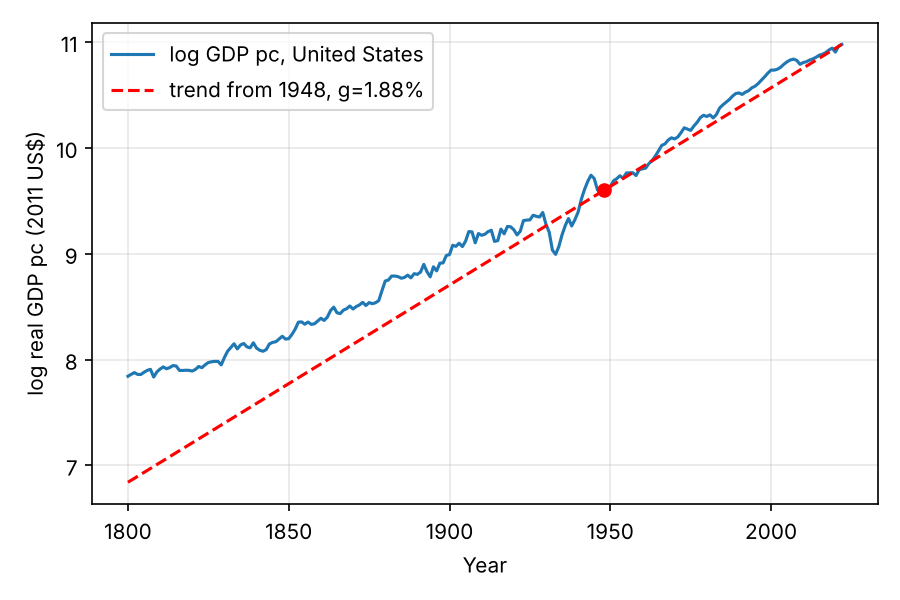
\includegraphics[width=0.75\textwidth]{fig_us.png}
\end{figure}
Observations: $\log y_t$ rises roughly linearly over two centuries, i.e.\ roughly constant exponential growth. The Great Depression (1929--33) and the sharp WWII boom and post-war fall (1940s) are the big deviations. After 1948 GDP pc stays close to the 1.88\% trend line, with small cycles around it (above trend in the 1960s and the late 1990s--2000s, below it in the 1970s--80s, and dips in 2008--09 and 2020), and ends almost exactly on it in 2022. I extended the line back to 1800 to show what the post-1948 growth rate would imply for the earlier period: it would put 1800 income at about \$935, well below the actual \$2,545, so growth before 1948 was slower than 1.88\% per year on average (the same point as in Section 1, parts 8--9).

\item \textbf{Alternative country: Japan.} Japan has data from 1948 to 2022: $y_{1948} = 2{,}857$, $y_{2022} = 38{,}269$, so $g = (38269/2857)^{1/74}-1 = 3.57\%$.
\begin{figure}[H]\centering
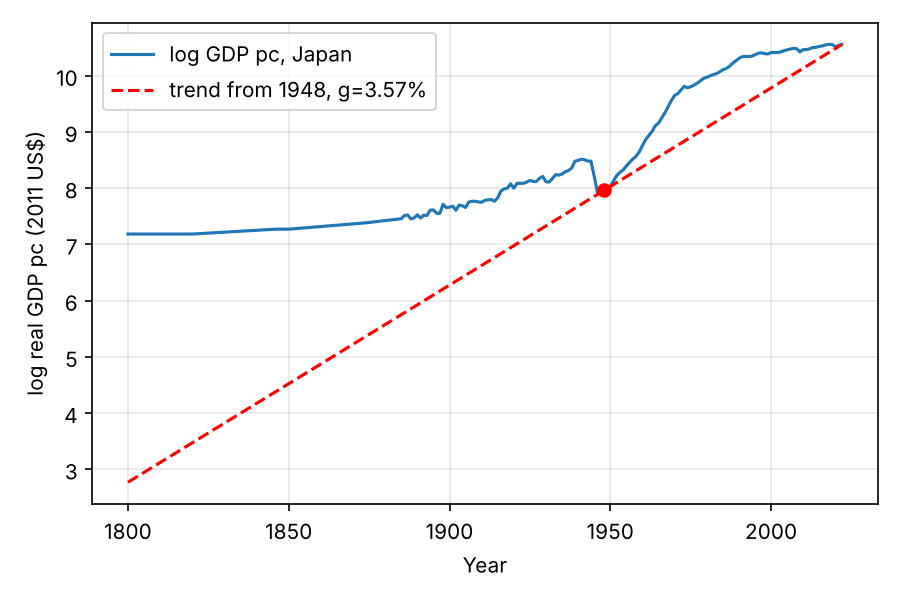
\includegraphics[width=0.75\textwidth]{fig_jp.png}
\end{figure}

\item \textbf{Comparison of slopes.} Japan's slope (3.57\%) is almost twice the U.S. slope (1.88\%). U.S.\ GDP pc rose by a factor of about 4.0 between 1948 and 2022, while Japan's rose by a factor of about 13.4. Japan started far behind (in 1948, in the aftermath of WWII, at about 19\% of the U.S.\ level) and caught up substantially: by 2022 it was at about 65\% of U.S.\ income. So living standards rose enormously in both countries, but much more in Japan, which is catching up. (The Japanese line also bends: very fast growth in the 1950s--1980s and slower growth since the early 1990s, so a single straight line fits less well than for the U.S.) Extended back to 1800, Japan's 3.57\% trend implies an income of only about \$16, versus the actual \$1,317, so Japan's postwar growth is far above anything in its earlier history.

\end{enumerate}

%==================================================================
\section{NIPA and Inflation}
%==================================================================

\begin{enumerate}[label=\textbf{\arabic*.}, leftmargin=*]

\item \textbf{Table IV and GDP (all in \$).}

\emph{Firm profits.} Krueger Bros.: total sales $100{,}000+60{,}000=160{,}000$, minus chicken purchases 50,000, wages 70,000, and sales taxes 20,000, gives profit of $20{,}000$. Freddy Chickens: $50{,}000-20{,}000-15{,}000-2{,}000 = 13{,}000$.

\emph{Households.} Wage income $=70{,}000+15{,}000+30{,}000 = 115{,}000$. Profits received $=20{,}000+13{,}000 = 33{,}000$. Total taxes collected are 30,000 and sales taxes paid by firms are $20{,}000+2{,}000=22{,}000$, so income taxes paid $=8{,}000$. Purchases of corn: total corn sales 100,000 minus 20,000 bought by Freddy $=80{,}000$. Purchases of chicken breast $=60{,}000$. Check: after-tax income $115{,}000+33{,}000-8{,}000 = 140{,}000 = 80{,}000 + 60{,}000$. \checkmark

\begin{table}[H]\centering
\begin{tabular}{lr}
\toprule
Wage Income & 115,000 \\
Income Taxes Paid & 8,000 \\
Profits Received from Firms & 33,000 \\
Purchases of Corn & 80,000 \\
Purchases of Chicken Breast & 60,000 \\
\bottomrule
\end{tabular}
\end{table}

\emph{Production approach} (sum of value added): Krueger $160{,}000-50{,}000 = 110{,}000$; Freddy $50{,}000-20{,}000 = 30{,}000$; Government $30{,}000$ (valued at cost). Total $=170{,}000$.

\emph{Expenditure approach:} $C = 80{,}000+60{,}000=140{,}000$, $G=30{,}000$, $I=0$, $NX=0$ (chickens and corn bought by the firms are intermediate goods). Total $=170{,}000$.

\emph{Income approach:} wages $115{,}000$ + profits $33{,}000$ + indirect (sales) taxes $22{,}000$ $=170{,}000$.

\ans{\text{Nominal GDP} = \$170{,}000 \text{ (all three approaches)}}

\item \textbf{Capital share of household income.}
Pre-tax household income is $115{,}000 + 33{,}000 = 148{,}000$, of which profits are $33{,}000$:
\[
  \frac{33{,}000}{148{,}000} \approx 22.3\%
\]
\ans{\text{Capital share} \approx 22.3\%}
(Relative to GDP it would be $33{,}000/170{,}000 = 19.4\%$.)

\item \textbf{Tax change.} Sales taxes paid by Krueger rise by 8,000 to 28,000, so its profit falls to $160{,}000-50{,}000-70{,}000-28{,}000 = 12{,}000$. Profits total $12{,}000+13{,}000=25{,}000$; wages are unchanged at $115{,}000$; sales taxes are $28{,}000+2{,}000=30{,}000$. Income approach:
\[
  115{,}000 + 25{,}000 + 30{,}000 = 170{,}000.
\]
\ans{\text{Nominal GDP} = \$170{,}000 \ (\text{unchanged})}
GDP is unchanged because the amount of output sold at market prices (and so the expenditure and production sides) is unchanged. The tax change only redistributes between income categories: the 8,000 that used to be income taxes on households (which are part of household income, and so already counted in wages and profits) now shows up as higher sales taxes, with profits falling by 8,000 while indirect taxes rise by 8,000.

\item \textbf{Laspeyres and Paasche price indices (2025 base).}
\begin{align*}
  P^L &= \frac{p^{26}_c q^{25}_c + p^{26}_b q^{25}_b}{p^{25}_c q^{25}_c + p^{25}_b q^{25}_b}
      = \frac{5(15{,}000)+6(5{,}000)}{4(15{,}000)+3(5{,}000)} = \frac{105{,}000}{75{,}000} = 1.400\\
  P^P &= \frac{p^{26}_c q^{26}_c + p^{26}_b q^{26}_b}{p^{25}_c q^{26}_c + p^{25}_b q^{26}_b}
      = \frac{5(20{,}000)+6(10{,}000)}{4(20{,}000)+3(10{,}000)} = \frac{160{,}000}{110{,}000} = 1.4545
\end{align*}
\ans{\pi^L = 40.0\%, \qquad \pi^P = 45.5\%}

\item \textbf{Fisher index.}
\[
  P^F = \sqrt{P^L P^P} = \sqrt{1.400 \times 1.4545} = 1.427
\]
\ans{\pi^F \approx 42.7\%}
Yes, the Fisher index must lie between the two: it is the geometric mean of $P^L$ and $P^P$, and the geometric mean of two positive numbers always lies between them (equal to both only if they are equal).

\item \textbf{Nominal and real GDP growth, 2025--2026.}
Nominal GDP: $2025$: $75{,}000$; $2026$: $160{,}000$. Growth $=160/75-1 =113.3\%$.
Real GDP should be measured at constant (2025) prices, i.e.\ deflated by the Paasche index (the GDP deflator): real GDP in 2026 is $160{,}000/1.4545 = 110{,}000$, which is $2026$ quantities at 2025 prices. Real growth: $110{,}000/75{,}000-1=46.7\%$. Equivalently $(1.1333+1)/ 1.4545 - 1$.
\ans{g^{nominal} \approx 113.3\%, \qquad g^{real} \approx 46.7\%}

\end{enumerate}

%==================================================================
\section{The Consumption-Saving Model}
%==================================================================

\begin{enumerate}[label=\textbf{\arabic*.}, leftmargin=*]

\item \textbf{Kate's budget constraints} ($r=0$, $a_0=0$):
\[
  c_0 + a_1 = w_0 = 100{,}000, \qquad c_1 + a_2 = a_1, \qquad c_2 = a_2 .
\]
Intertemporal budget constraint (substituting out $a_1, a_2$):
\[
  c_0 + c_1 + c_2 = 100{,}000 .
\]

\item \textbf{Lagrangian and Euler equation.}
\[
  \mathcal L = \log c_0 + 0.4\log c_1 + 0.16\log c_2 + \lambda\,[\,100{,}000 - c_0 - c_1 - c_2\,]
\]
FOCs: $1/c_0 = \lambda$, $0.4/c_1 = \lambda$, $0.16/c_2=\lambda$. Hence
\[
  \frac{1}{c_0} = \frac{0.4}{c_1}, \quad \frac{1}{c_1} = \frac{0.4}{c_2}
  \quad\Longrightarrow\quad c_1 = 0.4\,c_0, \quad c_2 = 0.4\,c_1 = 0.16\,c_0 .
\]
\ans{c_{t+1} = \beta(1+r)\,c_t = 0.4\,c_t}

\item \textbf{Kate's optimal choice.}
$c_0(1+0.4+0.16) = 100{,}000 \Rightarrow c_0 = 100{,}000/1.56$.
\[
  \boxed{c_0 \approx 64{,}103,\ c_1 \approx 25{,}641,\ c_2 \approx 10{,}256,\ a_1 \approx 35{,}897,\ a_2 \approx 10{,}256}
\]

\item \textbf{Pippa.} Euler: $c_1 = \tfrac23 c_0$. Budget: $c_0+c_1 = 100{,}000$, so $\tfrac53 c_0 = 100{,}000$.
\[
  \boxed{c_0 = 60{,}000,\ c_1 = 40{,}000,\ a_1 = 50{,}000 - 60{,}000 = -10{,}000}
\]
Kate consumes more in period 0 (64,103 vs.\ 60,000) even though both have lifetime income of 100,000. Kate is less patient ($\beta=0.4$ vs.\ $2/3$), and she has a longer horizon, so the share of wealth devoted to $c_0$ is $1/(1+\beta+\beta^2) = 64.1\%$ versus $1/(1+\beta) = 60\%$ for Pippa. Pippa is a \emph{borrower} ($a_1<0$): she wants to consume more than her period-0 income of 50,000 and smooth consumption. Kate is a \emph{saver} ($a_1>0$): all of her income arrives in period 0 and she must save to finance consumption in periods 1 and 2.

\item \textbf{Kate and the interest rate rise to 50\%.}
Now $c_1 = \beta(1+r)c_0 = 0.6\,c_0$ and $c_2 = 0.6\,c_1 = 0.36\,c_0$. The intertemporal budget constraint is $c_0 + c_1/1.5 + c_2/1.5^2 = 100{,}000$, and substituting:
\[
  c_0\,[\,1 + 0.6/1.5 + 0.36/2.25\,] = c_0\,[\,1+0.4+0.16\,] = 100{,}000 .
\]
\ans{c_0 = 64{,}103 \ (\text{unchanged})}
With log utility, the substitution effect (saving is more rewarding, so $c_0$ falls) exactly offsets the income effect (Kate is a saver and so is richer, so $c_0$ rises); the Euler equation shifts $c_1,c_2$ up, but the share of lifetime wealth spent on $c_0$ is independent of $r$.

\item \textbf{Pippa's response.} With $r=0.5$: Euler $c_1 = \tfrac23(1.5)c_0 = c_0$; present value of income $=50{,}000+50{,}000/1.5 = 83{,}333$; $c_0(1+1/1.5) = 83{,}333 \Rightarrow c_0 = 50{,}000$ (down from 60,000).
\ans{\text{Pippa's } c_0 \text{ responds more (falls 16.7\%) than Kate's (unchanged)}}
Pippa also has log utility, so (as for Kate) the substitution effect and the pure interest-rate income effect offset each other. But Pippa is a \emph{borrower}, and her income arrives partly in period 1: the higher rate lowers the present value of her lifetime income (from 100,000 to 83,333), so her wealth falls and so does $c_0$, whereas Kate's present value of income (all in period 0) is unaffected.

\item \textbf{Meghan.} Euler: $\tfrac32\cdot\tfrac12 c_0^{-1/2} = (1+r)\tfrac12 c_1^{-1/2} \Rightarrow c_1/c_0 = \tfrac49(1+r)^2$. At $r=0$: $c_0 = 25{,}000\cdot 2/(13/9) \approx 34{,}615$ (a borrower). At $r=0.5$: $c_1=c_0$, PV of income $=41{,}667$, $c_0 = 25{,}000$. (A fall of 27.8\%.)
\ans{\text{Meghan's response is stronger than Pippa's and Kate's}}
\emph{Versus Kate:} Kate's response is zero because log utility (elasticity of intertemporal substitution $=1$) makes income and substitution effects cancel for a saver, whereas Meghan is a borrower and also has a different curvature. \emph{Versus Pippa:} both are borrowers with the same relative discount factor $\beta=2/3$, so the income effect is similar; but Meghan's utility $\sqrt c$ is less curved than log (intertemporal elasticity of substitution of $2>1$), so she is more willing to substitute consumption across time and the substitution effect (a higher return on saving, so consume less now) is stronger. In percentage terms her $c_0$ falls by more (27.8\% vs.\ 16.7\%), though in dollars Pippa's drop (10,000) is slightly larger than Meghan's (9,615) since Pippa's income is twice as large.

\end{enumerate}

\end{document}
